\chapter{Workshop results}
\label{WorkshopResults}
As it is elaborated on in \autoref{ChapterWorkshop}, the purpose of the card sort and workshop is to elicit mental models of the users' interaction with a TonePrint community platform. In the workshop this is investigated for two specific tasks, which on their own don't provide a full explanation for how the entire information architecture should be. The given tasks are the overall new features going from the current TonePrint app to a TonePrint community, and the results are as such also overall explanations. For further elaborating explanations, the various elements in each task should be investigated on their own as a set of subtasks. The subjects' mental models are derived from their hand drawn concept maps and subsequent explanations of them, which was video recorded, and the purpose of the following chapter is to present the results of this workshop before uniting them with the results of the card sort.

\section{The individual task}
\label{IndividualTaskResults}
The workshop was conducted in a meeting room at TC Electronic's headquarters in Aarhus, and five members of their staff served as subjects for this. It's important to note that none of them have been affiliated with either the development or maintenance of the TonePrint application at any point, so they were considered fitting subjects for the workshop. The obvious bias of including developers of the TonePrint app would have meant that the workshop wouldn't have produced mental models representing those of the end-users. One of the subjects, however, was considered a potential bias as he develops templates for User TonePrints. He has not had any influence on the design of the TonePrint app though, so he was included in the individual task any way but instead served as an observer for the group task, leaving the remaining four subjects for this.

For the individual task, the results produced five different hand drawn concept maps, these are all found in \autoref{App:WorkshopConceptMaps}. The results for the subjects are presented individually including their concept map, depicted with software to make it more presentable and readable, a table of their highlighted content and actions, and codings of their video presentations. For the depicting of the concept maps it was considered insufficient to create a complete remake of their drawings alone, as they differ greatly in terms of structure and detail. In order to balance these differences, the new concept maps are made from their presentation of their drawings. The major pieces of content such as sites, list etc. are depicted in rectangles, while the components within this content, such as search, filtering etc. are depicted in rounded rectangles. The connections and actions between these elements are depicted as pointers. The codings of their explanations are presented with the concept map with the important content and actions highlighted with \textbf{bold text}. This is done to put the content and actions into context and not only have them displayed in a table.

\subsection*{Subject 1}
\label{Subject1}
Subject 1 starts from the \textbf{TonePrint app} where he wants to \textbf{Log in} in case he isn't already. Then he enters his \textbf{my TonePrints site} which contains a tab either called \textbf{friends}, \textbf{community} or something more fitting. He presses this tab and is redirected to either a \textbf{search friends} functionality or simply a \textbf{friends list}. The two could also be combined to include the search functionality within the friends list. He uses the search functionality by writing \textbf{user 1}, so it is the only name in the list, and by pressing the username he enters his \textbf{profile}. On this profile he is presented a \textbf{list of TonePrints} created by user 1. The list is divided into the tabs \textbf{by name} and \textbf{by type}. From the list of types, he selects the \textbf{Corona TonePrints} and under this he wants to select \textbf{Warm Corona}. This selection could either be confirmed by an \textbf{add to my list} option or a button with a gear symbol on it, even though he's not completely sure what would happen by pressing it. Instead he proposes pressing the name of the TonePrint which would unveil a heart, giving him the choice of \textbf{liking} the TonePrint. It would also present him with instructions in the shape of \textbf{about}, \textbf{how i use it}, and \textbf{number of users}.\\
%
\begin{table}[H]
\begin{minipage}[b]{\linewidth}\centering
	\begin{tabular} {|l|l|l|} \hline
		\rowcolor{xGray25} \textbf{Content} & \textbf{Actions} \\  \hline
		TonePrint app & Logging in \\
		My TonePrints site & Pressing friends/community tab \\
		Friends/Community tab & Writing "user 1" \\
		Search functionality & Pressing user 1 name \\
		Friends list & Filter by type \\
		User 1 profile & Selecting Warm Corona \\
		List of TonePrints & Pressing "add to my TonePrints" \\
		Type and name filter & Pressing like functionality \\
		Corona TonePrints & \\
		Warm Corona & \\
		Like functionality & \\
		About this TonePrint & \\
		How i use this TonePrint & \\
		Number of users & \\ \hline
	\end{tabular}
	\caption{The important content and actions mentioned by subject 1}
	\label{tab:Subject1ContentActions}
\end{minipage}
\end{table}
%
\begin{figure}[H]
	\centering
	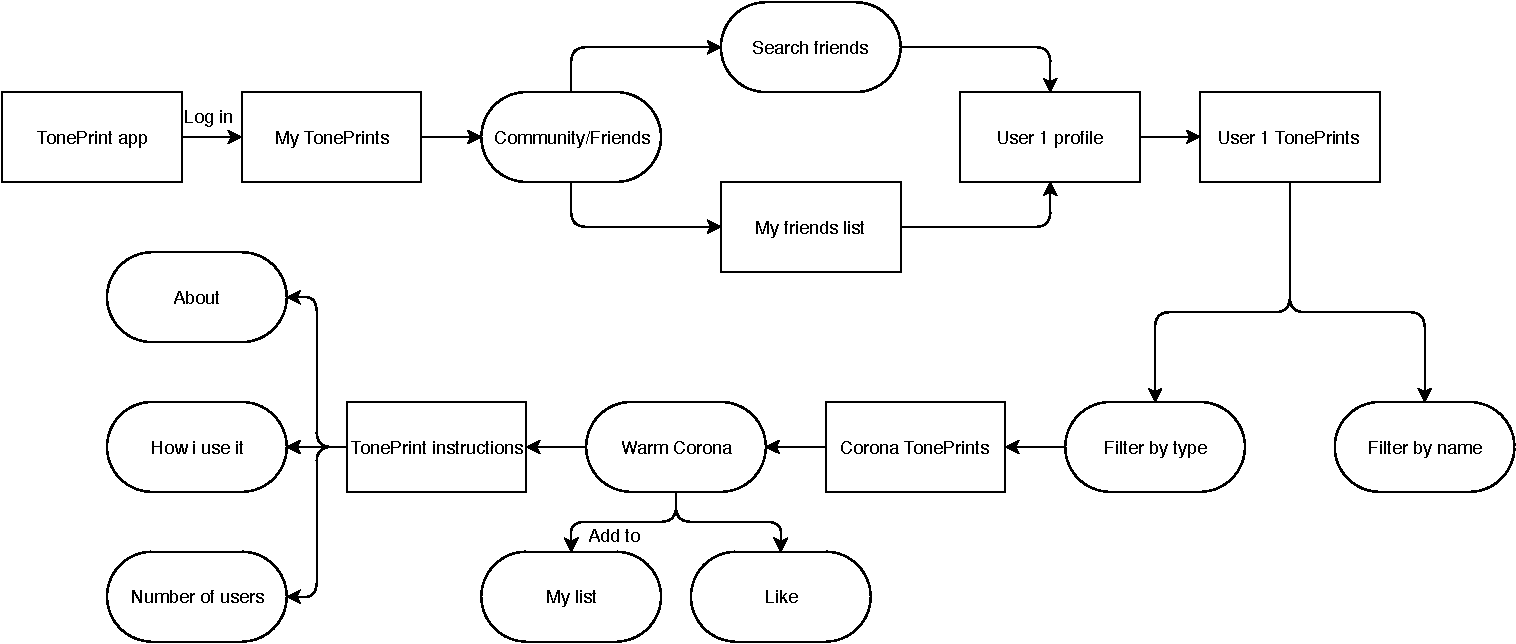
\includegraphics[width=\textwidth]{1ICMM_new.pdf}
	\caption{The Concept for subject 1. The hand-drawn version is displayed in \autoref{fig:DrawnICMM1}.}
	\label{fig:ICMM1}
\end{figure}


\subsection*{Subject 2}
\label{Subject2}
Subject 2 starts by opening the \textbf{TonePrint app}, after this he has two options. The user can either open his list of \textbf{subscriptions}, if he's looking for a user that he already has subscribed to, or he can open another \textbf{list} and simply \textbf{search} for user 1. Whatever the approach, the next step is then to hook up a pedal and guitar, and select one of \textbf{user 1's Corona TonePrints}. He selects one of them and \textbf{Loads it to his pedal}. Subject 2 then tries out the TonePrint by playing the guitar, and if doesn't like it, he goes back and selects a new TonePrint. If he does like the TonePrint, he wants to \textbf{highlight} it as one of his \textbf{favourites}, so he can find it at another time. He would also like to \textbf{store it in his pedal}. Finally, by selecting to subscribe to the user, he would expect the system to send him \textbf{notifications}, when the user uploads \textbf{new TonePrints}, either directly in the app or maybe by mail. When all these steps are clear, subject 2 would then expect to unhook the pedal from the app and start playing with the TonePrint in question. \\
%
\begin{table}[H]
\begin{minipage}[b]{\linewidth}\centering
	\begin{tabular} {|l|l|l|} \hline
		\rowcolor{xGray25} \textbf{Content} & \textbf{Actions} \\  \hline
		TonePrint app & Looking through "subscribed to" users \\
		Subscriptions list & Searching for user 1 \\
		Search list & Hook up pedal and guitar \\
		User 1 Corona TonePrints list & Selecting a user 1 TonePrint \\
		Favourites list & Loading TonePrint to pedal \\
		Notifications of new TonePrints & Trying out the TonePrint \\
		 & Highlight as favourite \\
		 & Storing TonePrint in pedal \\
		 & Unhook pedal from the app \\ \hline
	\end{tabular}
	\caption{The important content and actions mentioned by subject 2}
	\label{tab:Subject2ContentActions}
\end{minipage}
\end{table}
%
\begin{figure}[H]
	\centering
	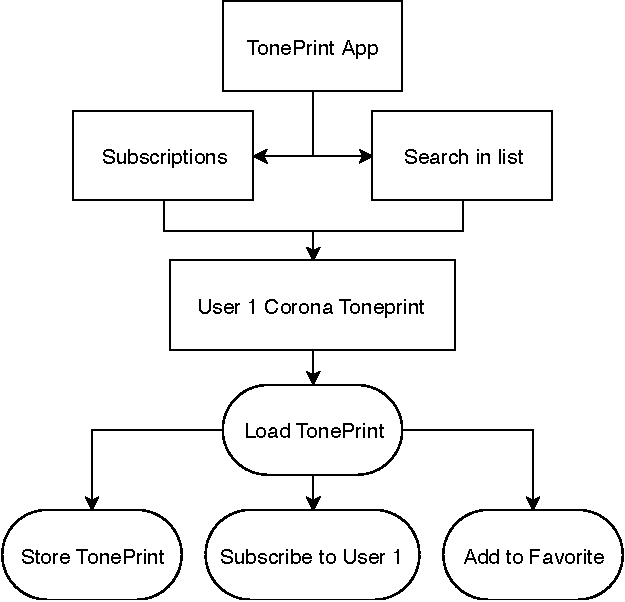
\includegraphics[width=0.9\textwidth]{2ICMM_new.pdf}
	\caption{The Concept map for subject 2. The hand-drawn version is displayed in \autoref{fig:DrawnICMM2}.}
	\label{fig:ICMM2}
\end{figure}


\subsubsection{Subject 3}
\label{Subject3}
Subject 3 starts by opening the \textbf{TonePrint app} and gets a \textbf{notification} telling him that user 1, who he already \textbf{subscribes} to, has uploaded a new \textbf{Chorus TonePrint}. He tabs this notification, sending him directly to the specific \textbf{Chorus TonePrint site}, where he selects \textbf{save TonePrint}. From here he can then go to \textbf{user 1's profile} where he can check out other \textbf{TonePrints made by user 1}. He expects these to be sorted in a \textbf{logical order} such as \textbf{alphabetically} or something more fitting. \\
%
\begin{table}[H]
\begin{minipage}[b]{\linewidth}\centering
	\begin{tabular} {|l|l|l|} \hline
		\rowcolor{xGray25} \textbf{Content} & \textbf{Actions} \\  \hline
		TonePrint app & pressing notification \\
		Notification system & Saving TonePrint \\
		Chorus TonePrints & pressing user 1's profile name \\
		Chorus TonePrint site &  \\
		User 1 profile &  \\
		User 1 TonePrint list &  \\
		Alphabetical sorting &  \\ \hline
	\end{tabular}
	\caption{The important content and actions mentioned by subject 3}
	\label{tab:Subject3ContentActions}
\end{minipage}
\end{table}
%
\begin{figure}[H]
	\centering
	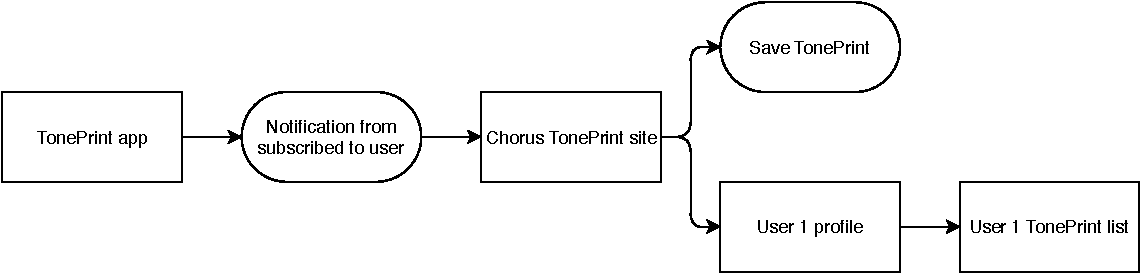
\includegraphics[width=0.9\textwidth]{3ICMM_new.pdf}
	\caption{The Concept for subject 3. The hand-drawn version is displayed in \autoref{fig:DrawnICMM3}.}
	\label{fig:ICMM3}
\end{figure}


\subsubsection{Subject 4}
\label{Subject4}
Subject 4 starts by opening the \textbf{TonePrint app} which he expects to have the same infrastructure as the current TonePrint app. He then navigates to \textbf{User TonePrints} where he expects to find all of his own TonePrints as well as an option called \textbf{cloud library}. By selecting this, he is redirected to where \textbf{all user TonePrints} are stored, and he wants find a TonePrint from a user that he already knows. He expects there to be a \textbf{filtering system} of some sort, and he chooses to \textbf{filter by product}, presenting him with a list of all \textbf{cloud based Corona TonePrints}. Subject 4 would then like to \textbf{search} for user 1, redirecting the list to the Corona TonePrints made by user 1. An alternative approach would be to just search for user 1 in the first place and be presented for all \textbf{user 1 TonePrints}. He considers this a more direct approach, as it only requires one action, but by using the current infrastructure of the TonePrint app, he would expect the filtering system to be a part of the solution. Subject 4 then enters \textbf{User 1’s profile}, where he is presented the TonePrints of user 1, although just the Corona types given the filtering system. He then clicks on a TonePrint with the intention of \textbf{trying it out in real time}, indicating that he wants to \textbf{transfer the TonePrint to his pedal}. If he then likes it, he can choose to \textbf{save it to his own library} and \textbf{highlight it as a favourite}. He wants an interface like the current TonePrint app, where he can \textbf{Save the TonePrint} and \textbf{Store it in pedal}. \\
%
\begin{table}[H]
\begin{minipage}[b]{\linewidth}\centering
	\begin{tabular} {|l|l|l|} \hline
		\rowcolor{xGray25} \textbf{Content} & \textbf{Actions} \\  \hline
		TonePrint app & Selecting cloud library \\
		User TonePrints & Filter by product \\
		Cloud library & Searching for user 1 \\
		List of all user TonePrints & Clicking on a Corona TonePrint \\
		Filtering system & Trying TonePrint in real time \\
		Cloud based Corona TonePrints & Transfering TonePrint to pedal \\
		Search functionality & Saving TonePrint to his own library \\
		User 1 Corona TonePrints & Highlighting TonePrint as a favourite \\
		All user 1 TonePrints & Saving the TonePrint \\
		User 1 profile & Store TonePrint in pedal \\ \hline
	\end{tabular}
	\caption{The important content and actions mentioned by subject 4}
	\label{tab:Subject4ContentActions}
\end{minipage}
\end{table}
%
\begin{figure}[H]
	\centering
	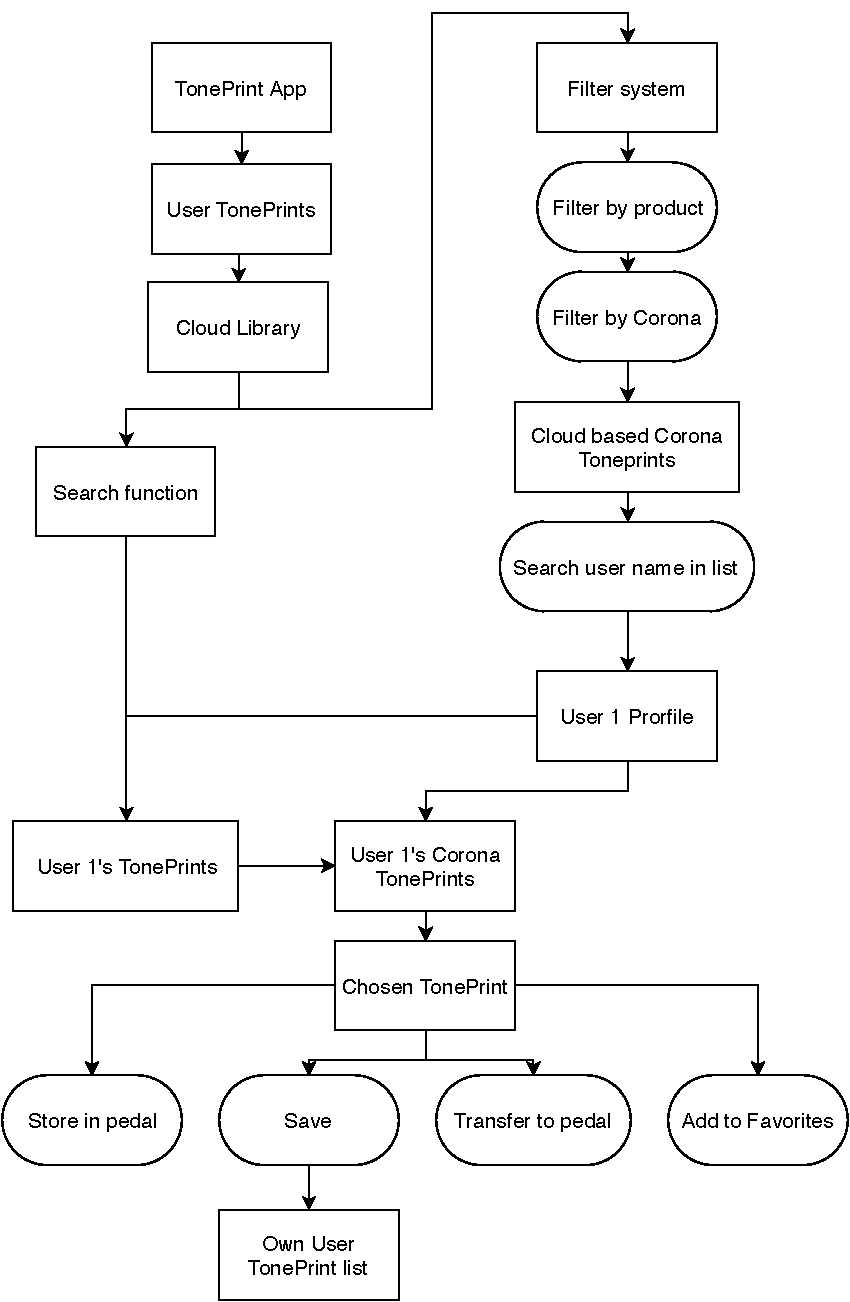
\includegraphics[width=\textwidth]{4ICMM_new.pdf}
	\caption{The Concept map created by subject 4.}
	\label{fig:ICMM4}
\end{figure}


\subsubsection{Subject 5}
\label{Subject5}
Subject 5 starts by saying it needs to feel as familiar as possible, \textbf{similar to other apps} such as Youtube. Everyone uses these, and they tend to be somewhat similar. In the \textbf{TonePrint app} he therefore imagines a \textbf{magnifying glass icon} in the corner for \textbf{searching}, and he further proposes an \textbf{advanced search} for personalising the search. In either case, he proposes that it should work as a \textbf{meta search option}, where everything fitting to the search criteria within the system is presented to the user. In order to present this more organised, he proposes \textbf{different icons representing different content}. In the case of searching for user 1, the system would then provide a \textbf{suggested user: user 1}. By pressing this, the user is then redirected to all the \textbf{public content for user 1}, \textbf{sorted by products}. From here, he selects \textbf{Corona TonePrints} which unveils a \textbf{miniature view} of all user 1's TonePrints for this product, and when selecting one of these, the user is presented a site with all the \textbf{TonePrint details} and maybe a \textbf{picture} attached to the description. Should he just right click on it or hold a finger on it on the smartphone version, he would see a \textbf{context menu} with the options: \textbf{Beam}, \textbf{clone}, or \textbf{add to personal library}, allowing him to \textbf{edit it} or \textbf{highlight it as a favourite}. Finally, he describes a \textbf{history functionality} which allows him to \textbf{backtrack his actions}, much like in a web browser. As such, he will be able to find a TonePrint, even if he didn't highlight it as a favourite \\
%
\begin{table}[H]
\begin{minipage}[b]{\linewidth}\centering
	\begin{tabular} {|l|l|l|} \hline
		\rowcolor{xGray25} \textbf{Content} & \textbf{Actions} \\  \hline
		Similar to other apps & Pressing magnifying glass \\
		TonePrint app & Searching for user 1 \\
		Magnifying glass icon & Pressing suggest user: User 1 \\
		Search functionality & Selecting Corona TonePrints \\
		Advanced search & Selecting a specific TonePrint \\
		Meta search & Right clicking / holding a TonePrint \\
		Different icons for different content & adding to personal library \\
		Suggested user: User 1 & Further editing the TonePrint \\
		Public content for user 1 & Highlighting as favourite \\
		Corona TonePrints & Backtracking his actions \\
		Miniature view &  \\
		TonePrint details & \\
		Picture with the description & \\
		Context menu & \\
		Beaming option & \\
		Clone option & \\
		Add to personal library & \\
		Favourite option & \\
		Edit option & \\
		History functionality & \\ \hline
	\end{tabular}
	\caption{The important content and actions mentioned by subject 5}
	\label{tab:Subject5ContentActions}
\end{minipage}
\end{table}
%
\begin{figure}[H]
	\centering
	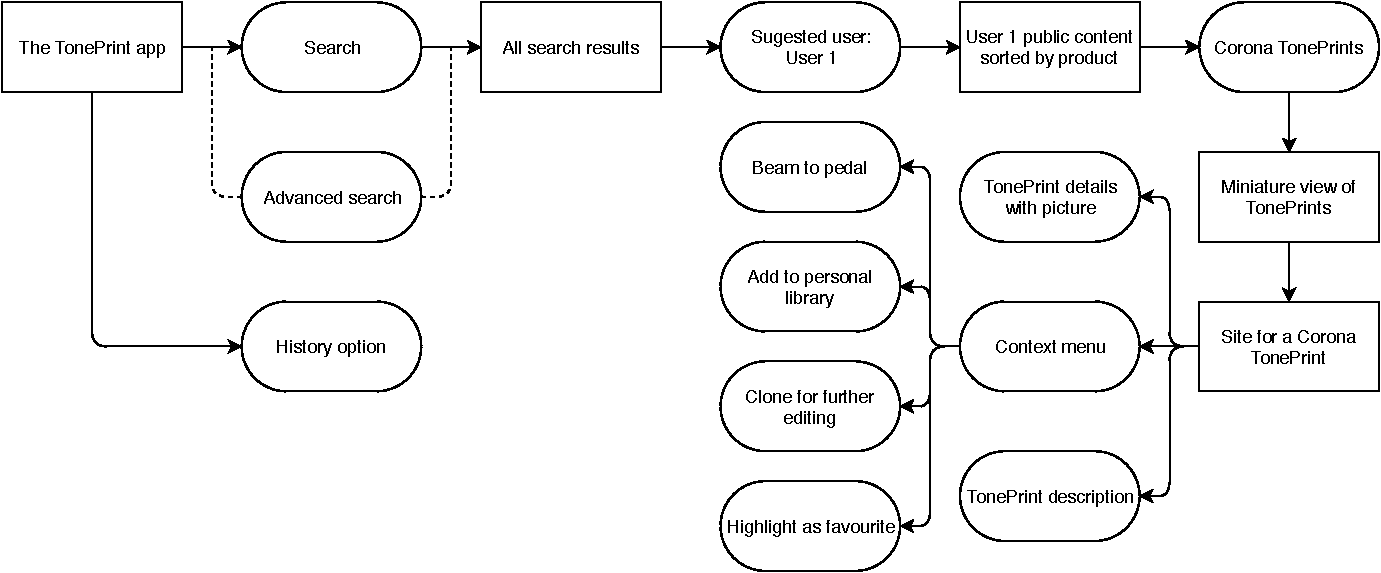
\includegraphics[width=0.4\textwidth]{5ICMM_new.pdf}
	\caption{The Concept map created by subject 5.}
	\label{fig:ICMM5}
\end{figure}



\section{Reflecting on the task results}
\label{IndividualTaskReflection}
Before investigating the results of the group task, it seems fitting to first take a look at the results of the individual task in order to find common traits between the subjects. Had the workshop provided no major differences between them, then it would seem more or less straightforward, how the design of the information architecture should be approached, but this is not the case. It's also important to note that only 5 potential end-users participated as subjects in the workshop, and conducting more workshops with more subjects could just as well provide other results.

All the subjects start the same way by opening the TonePrint app, with subject 4 even stating that he would expect to start from the current TonePrint app with the same infrastructure. They weren't instructed to approach the task on the basis of the current TonePrint app and the TonePrint community as one unit, but this might be due to bias from the task example. The route they then chose to reach the TonePrint made by user 1 turned out be rather different. Subject 1 and 4 propose they start by entering their own site of User TonePrints, where they have a tab giving them access to the public User TonePrints. subject 1 refers to this as \textit{friends} and \textit{community}, while subject 4 refers to it as \textit{cloud library}. For subject 2 and 5 it seems as the current app and community are completely unified, as they jump straight to a search functionality with subject 2 also proposing to enter a list of users that he already subscribes to. Subject 3 has the fastest route to the TonePrint of them all. He also proposes a subscription system, but in his version he receives a notification of a new TonePrint by user 1 that redirects him straight to it, skipping a lot of steps included by the other subjects.

Subject 1 and 4 then proposes a search functionality as well. Subject 4 first want to filter the vast amount of TonePrints by product, but both of them, as well as subject 2 and 5, wants to write "user1" and press the search result. This points towards that a search functionality should be included, even though it's not completely clear how the action itself and subsequent search results should be presented, and how advanced it should be. From the search there also seems to be some difference to where the subjects then expect to be redirected to. Subject 2, 4, and 5 expects to be taking directly to a list of all the TonePrints for user 1, with subject 5 referring to it as all the public content for user 1. Subject 1 expects to be taken to a profile for user 1, and this concept of a profile is present for more subjects, but he is the only one expecting to be taken to it at this point. In reality, all except subject 2 mentions a profile at some point during their presentation, and this would imply that profiles should in some way be a part of the TonePrint community.

When reaching the correct TonePrint, the subjects generally have the same idea of what to do next. all subjects except subject 3 wants to highlight it as a favourite, and subject 1, 4, and 5 also wants to save or add it to their own TonePrint library while subject 2 and 4 talks about storing the TonePrint to the pedal. Subject 2 and 4 furthermore want to play with the TonePrint in real time before deciding on whether to save it or not. As final remarks, the subjects also proposed content for the TonePrint community such as backtracking options, further editing the saved User TonePrints, and proper instructions for the TonePrint, including how to use it and its number of users.


\section{Group task result}
\label{GroupTaskResults}
For the group assignment the participants were asked to work as a team to generate a map of how the given task should be solved in order to reach the end goal. One of the participants was excluded for this assignment because he were found to biased, on the account of his work. For the group assignment his knowledge could have had a to large affect on the end result in a way that it would reflect a developers mental model rather than a end users.\\ 
Compared to the results of the individual assignment is the scope for the group assignment to let the participants discuss how the system should work in order for them to reach the goal. This should give a more reflective answer because the participants need to reach an agreement.\\

\noindent
For the process of making the parameter settings they find agree upon the current system is suitable and that after the TonePrint settings has been set the TonePrint is given a name. However for the description and tagging part the current system isn't sufficient. It's argued that both the description and the tags aren't necessary if the user doesn't want to share the TonePrint and only wants to use it  by himself. For the purpose of sharing ones TonePrint several thing are discussed in accordance to both description and tags. One thing overall is the distinction between description and tags, because they may have a lot in common in terms of purpose. They are both seen as a tool that describes the TonePrint. One participant even argues that the tags might even be included in the description, maybe in the shape of Hashtags. For the description they want it to be something that the user writes themselves in when the TonePrint is to be shared, when its not the system shouldn't force one to include it. One also argues that it should be allowed to include a picture in the description. \\
When the participants are discussing tags it mostly focus around two ways of doing it. They suggest that after one have written the description the system should should present a list of "Suggested Tags". These suggested tags would be generated by the system and based on the settings of the TonePrint. It's also suggested that the system could use the user written description to generated suggested tags. When talking about suggested tags they imagines that it would be based on and thereby create tags describing Genre, Effect type, Settings of the TOnePrint, Description and Craziness, which describes if a setting is set at extreme levels. It's argued that the suggested tags could be automatically applied, while another argue that it could be suggested through a drop down menu. After the suggested they describe that it should be possible to create one's own tags, in the case of the suggested not being sufficient. \\
After tagging they are discussing how they would like to be able to share the TonePrint. At the beginning it's seen as a simple function which just said "Public", but than it's argued that it could be nice if it was possible to be able to share one's TonePrint on other media as a link e.g. Facebook or via mail. This leads to a discussion of how it could be shared with e.g. band members, but at the same time not having it as a public TonePrint. The participants suggest two ways of sharing the TonePrint. Firstly there is the "Public" function, which allows every one to find the TonePrint by e.g. searching on the tags used to describe the it. The other solution is inspired by the smart-phone app Snapchat, whereas it's possible to send it to individual friends or to a group. This leads to three situations the participants suggest the TonePrint can end in. The TonePrint can be kept Private, so that it's only accessible to the created, it may end in the category the participants name "Unlisted" meaning its accessible for the created and the selected people he shares it with and will not appear if search upon by others. Lastly it could be categorized as public which means it's accessible to every one and it appears when search upon. When the TonePrint is public it suggested that one still should be able to share it with friends and groups of one's choosing.\\


\section{Reflecting on group task}
\label{GroupTaskReflection}
To quickly summarize the model created during the group discussion.\\
At first the TonePrint app is opened and a TonePrint i created and is given a name. Hereafter the user can save if he doesn't want to share it, however in this case he want to and therefore goes chooses to write a description of what what he think the TonePrint is useful fore and maybe add a picture of his band or his setup. Here after the system suggests a number of tags based on the TonePrint and the description he written. Hereafter the user have the option to add extra tags if he wishes to. After applying the desired tags the user has completed the TonePrint and shall choose the privacy settings of it. If he have regret to share it yet, he may select the "private" setting. If he want to just share it with his band and maybe a friend or two he can select the "Unlisted" setting and then send it to those he wishes. Finally he may select the "Public" setting, making in accessible for every other user, and still send it to those i want.


























%\subsection{Shared Analysis}
%\label{SharedAnalysis}
%%
%The next phase is the shared analysis in which the codes derived from the ICMM's is used, in order to find items (concept and links) which is shared between them. In order to determine which items that identifies as shared a criterion needs to be defined. As described in \autoref{ACSMM} it's suggested to set the criterion at 50\% at the beginning, which afterwards may be adjusted. This means that a given item have to occur in atleast in 50\% of the ICMM's to be identified as shared.\\
%To compare the codes they are first typed into tables, for the purpose of gathering the codes for easier overview. The tables containing the codes is \autoref{tab:Subject1Coded} to \autoref{tab:Subject5Coded}. 
%
%The lists containing the subjects individual codes, \autoref{tab:Subject1Coded} to \autoref{tab:Subject5Coded} are compared to each other to find the concepts which is shared. As recommended by \textcite{WEB:ConceptMapAnalysis} is the criterion for a concept to be identified as shared defined as 50\%. The concepts which is defined as shared is listed at \autoref{tab:SharedConcept}(WHich isn't finish). 
%
%It's deemed problematic to use the described steps from \textcite{WEB:ConceptMapAnalysis} to create a ACSMM. This is because the task of the workshop was for the subjects to solve a task with a they have to build up as they go. This gives the users full control in regards to which features that exists in the system, how they works and when they wants to use them. This results in the subjects going different ways around the task and solving it in their won way. This is quite similar to some system in the real world which give you the option to reach a certain goal different ways. This however creates one big problem regarding, them only describing the part of the system, which they uses. This makes it very difficult to compare one persons ICMM with another, because they may have chosen different ways of solving the task and theirby having a minimal of similar concepts in common. This doesn't necessarily mean that the two subject disagree on how the system should work and their mental models might be similar towards the system. They just have chosen different approaches for the task, ehich means that they don't uses the same branches of the system. \\
%
%\begin{table}[]
%	\centering
%	\begin{tabular}[width=\textwidth]{c|lllllc}
%\hline 
%Shared item & subject 1 & subject 2 & subject 3 & subject 4 & subject 5 & \%	\\ \hline
%TP App & TP App & App & TP App & TP App & TP App & 100\%	\\ 
%My User Toneptints & My TonePrint site &  &  & User TonePrints \& Own User TonePrint Library & Personal Library & 60\% \\
%Search function & Search Friends & Search in List & & Search User Name \& Search Function & Search, Advanced search \& Meta Search Option & 80\% \\
%User 1 Profile & User 1 Profile & & User 1 Profile & User 1 Profile site & & 60\% \\
%User 1 TonePrints & User 1 TonePrint list & & User 1's Toneprints & User 1 TonePrints
%	\end{tabular}
%\end{table}
%
%\begin{table}[H]
%	\centering
%	\begin{tabular}[width=\textwidth]{|l|c|}
%	\hline
%	Shared concept & Sharedness level (\%) \\ \hline
%	TP App & 100\% \\ 
%	User TonePrint Library & 60\% \\ \hline
%	\end{tabular}
%	\caption{Shared concepts and sharedness level}
%	\label{tab:SharedConcept}
%\end{table}














